\documentclass[12pt]{beamer}

% Turn off the ugly navigation symbols.
\setbeamertemplate{navigation symbols}{}

% Margins and whatnot.
\setbeamersize{text margin left=2em,text margin right=2em}

\usepackage{fontspec}
\defaultfontfeatures{Mapping=tex-text} % enable -- / --- / `` / ''
\usefonttheme{serif}
\setmainfont{Helvetica}
\setsansfont{Oswald}
\setmonofont{Courier}

\definecolor{verydarkgrey}{HTML}{001112}
\definecolor{darkblue}{HTML}{232747}
\definecolor{grey}{HTML}{777777}

\setbeamerfont{frametitle}{size=\Large}
\setbeamercolor{frametitle}{fg=black}
\setbeamercolor{titleline}{bg=black}
\setbeamercolor{title}{fg=black}
\setbeamercolor*{date in head/foot}{fg=grey}
\setbeamercolor{item}{fg=black}
\setbeamerfont{item}{series=\bfseries}
% Never used, but this is nice.
\setbeamertemplate{itemize subitem}{--}
\setbeamerfont{itemize/enumerate subbody}{size=\small}

% \useoutertheme{new}

\makeatletter
\usepackage{dashrule}
\defbeamertemplate*{frametitle}{mine}[1][left]
{
  % Increase width of title box
  \@tempdima=\textwidth%
  \advance\@tempdima by\beamer@leftmargin%
  \advance\@tempdima by\beamer@rightmargin%
  %
  \begin{beamercolorbox}[sep=0.3cm,#1,wd=\the\@tempdima]{frametitle}
    \usebeamerfont{frametitle}%
    \vbox{}\vskip-1ex\vspace{.5ex}
    \strut\hspace{2ex}\sf\insertframetitle\strut\par%
    \vskip-1.5ex%
    \hspace{\fill}%
    %\hdashrule{\textwidth}{.075ex}{.075ex .2ex}%
    \color{black}{\rule{\textwidth}{.075ex}}%
    \hspace{\fill}%
    \par\nointerlineskip \vspace{\baselineskip}
  \end{beamercolorbox}%
  \nointerlineskip%
  \vspace{-3.5ex}
}

% \defbeamertemplate*{footline}{}
% {
%   \hbox{%
%   \begin{beamercolorbox}[wd=.8\paperwidth]{section in head/foot}%
%   \end{beamercolorbox}%
%   \begin{beamercolorbox}[wd=.2\paperwidth,ht=2.25ex,dp=1ex,right]{date in head/foot}%
%     \insertframenumber{} / \inserttotalframenumber\hspace*{2ex} 
%   \end{beamercolorbox}}%
%   \vskip0pt%
% }
\makeatother


\usepackage{fancyvrb}
\usepackage{fancyvrb}
\usepackage{xcolor}
\usepackage{relsize}
\newcommand{\code}{\texttt}
\usepackage{url}
\newcommand{\Rstar}{R$^*$}
\newcommand{\ud}{\mathrm{d}}

\newcommand{\wikipic}[1]{%
\begin{center}%
\includegraphics[width=.8\textwidth]{figure/simple_models_#1}%
\end{center}}
\newcommand{\wikipich}[1]{%
\begin{center}%
\includegraphics[height=.8\textheight]{figure/simple_models_#1}%
\end{center}}
\newcommand{\subt}[1]{{~~~\normalsize (#1)}}

\usepackage[overlay,absolute]{textpos}
\newcommand\FrameText[1]{%
  \begin{textblock*}{\paperwidth}(0pt,\textheight)
    \raggedleft #1\hspace{.5em}
  \end{textblock*}}

\begin{document}

% Need a nice title slide.  Probably just go with a picture and the
% text in a box.  Simple and relatively easy.  Picture could just be a
% tropical forest shot or something, or a slide split between a
% tropical forest and a monoculture of some sort, which would lead
% into the next slide nicely.
\begin{frame}
  \thispagestyle{empty}
  \begin{center}
    \sf
    {\Huge Competition Kernels \& Coexistance}\\[2ex]
    % {\footnotesize {}}\\[1.5em]
    {\large Rich FitzJohn, Daniel Falster,\\[1ex]
    Georges Kunstler, Mark Westoby}
  \vfill
  [these are notes slides and actual interesting slides coming later]
  \end{center}
\end{frame}

\begin{frame}
  % I'm going to need an intro hook.  Previously I drove things from
  % "competition is a homogenising and a disruptive force", but
  % suggestion in lab meeting was to start with limiting similarity.
  %
  % One option is to put the figure from hermoyian 2002 in (bivales
  % across a gradient) and the finch things.  That'd be nice if I then
  % have a finch figure.
  %
  % Another way is to start with "models of competition make it into
  % many different types of evolutionary models: of coexistance, trait
  % evolution, character displacement, dispersal, etc".  Competition
  % can be a homogenising force leading to competitive exclusion or it
  % can generate disruptive selection allowing for many different
  % types to coexist by deforming the fitness landscape.
  %
  % 
  % > On the one hand, competition is a homogenising force -- winner
  % > takes all is one extreme end of competition.  So competition can
  % > lead to a lack of divesity. [picture of grass? beech forest?]
  %
  % > On the other hand, competition a diversity-generating force -- it
  % > can generate disruptive selection that forces traits apart.
  % > Competition is present in almost all theory abaout how
  % > hyperdiverse systems come to be. [picture of tropical forest]
  %
  % However, the way that we model competition tends to be very
  % simple.
  \begin{center}
    [Intro stuff still undecided]
  \end{center}
\end{frame}

\begin{frame}
  % Despite the centrality of the idea, the way we model competition
  % is surprisingly simple.  When competition is assumed into a model,
  % we tend to reach for the simplest cases -- that's fine, but these
  % are usually variants on the MacArthur and Levins model from 1967,
  % itself a modification of the Lotka--Volterra models of the 30s.

  % Combination of logistic growth and the Lotka-Volterra equation.
  % Competition function maps species traits to how much they suppress
  % the growth and carrying capacity of other species.

  % Don't know why this won't fit better.  Increasing the width just
  % pushes the damn thing off the edge.  Check with eseb talk, though
  % I think I used tikz for all placement there.
  %
  % TODO: This set of figures should be a finch and seed sizes along
  % the bottom, and then the last one should have the plant leaves.
  %
  % TODO: Mention limiting similarity and pop a reference to Macarthur
  % here?  Possibly also the figure from that paper.
  \includegraphics<1>[width=\textwidth]{figs/gaussian_competition_1}
  \includegraphics<2>[width=\textwidth]{figs/gaussian_competition_2}
  \includegraphics<3>[width=\textwidth]{figs/gaussian_competition_3}
  %
  % TODO: At some point within this series, put the hermoyian 2002
  % figure and the finch figure here and point out that people
  % interpret these sorts of trait distributions are evidence for
  % competition.
  %
  % Then move to the leaf one and say that it's less clear how we
  % should interpret this for plants where the resource axis is less
  % clear.
\end{frame}

\begin{frame}
  % Plant ecology has become increasingly trait focussed over the last
  % few decades, and has moved from counting "species identity" as
  % important to trying identify major axes of functional variation.
  % We can point at things like the leaf economic spectrum and say
  % "That's a fast plant" and "that's a slow plant", but it's very
  % difficult to say anything *in general* about how these traits
  % might relate to competiton, and therefore to things like
  % coexistance.
  \includegraphics[width=\textwidth]{figs/bridge_1}
  % Around here, introduce the traits that we have information for,
  % possibly including a picture that represents SLA, hmat.
  % 
  % Perhaps: bunch of leaves with letters A - X on them, and
  % then recast as a series of points along the LMA / leaf lifespan
  % plot, coloured up.  So we want silhoettes I think.
\end{frame}

\begin{frame}{How do we model competition?}
  % Despite the centrality of the idea, the way we model competition
  % is surprisingly simple.  When competition is assumed into a model,
  % we tend to reach for the simplest cases -- that's fine, but these
  % are usually variants on the MacArthur and Levins model from 1967,
  % itself a modification of the Lotka--Volterra models of the 30s.

  % No need to go into the model in any detail, but just say that it
  % is a mix of the LV and logistic models, and list the assumptions:
  %
  % Competition intensity increases linearly with species density
  % ...directly summed over all species.
  \begin{itemize}
  \item Simple models, usually based model by MacArthur and Levins 1967.
  \item Combination of logistic growth and the Lotka-Volterra
    equations.
  \end{itemize}

  Implies competition will be
  \begin{itemize}
  \item constant with respect to densities of all species
  \item linear in species density
  \item linear over all species in the community
  \end{itemize}
  Gaussian usually gaussian in trait space
\end{frame}

\begin{frame}{How do we connect these models with real data?}
  %
  % Obviously models are not meant to be facsimilies of the real
  % world, but there are real issues here in connecting these sorts of
  % models to the real world.
  %
  % What I want to do here is look at how we can build a bridge
  % between these very simple models and the types of data that we
  % have, via mechanistic models.

  % About here: clarify "implicit" and "explicit" competition.
  \begin{itemize}
  \item Theoretical models framed in terms of \textbf{resource use};
    the ``trait'' is really preference for a resource.
  \item (finch and seed size preference picture)
  \item (picture of a tropical forest and a few plant traits)
  \end{itemize}
\end{frame}

\begin{frame}{Aims and Questions}
  % Much of the last point ends up here.
  % 
  % Emphasise the major research goal is to build the bridge, but the
  % current question is just to see what sort of competition kernels 

  \begin{itemize}
  \item What does competition kernels look like?
  \item Are the assumptions in the LV model reasonable?
  \item What would it take to build a bridge between theory and data
    that allows us to detect disruptive selection on traits?
  \item I don't actually have solutions for any of this.
  \end{itemize}

  Look at the competition kernels induced by one simple and one
  complicated model.
\end{frame}


\begin{frame}{Approach}
  % The approach we took was really simple minded: we focus on invasion
  % fitness (the fitness of a rare mutant with some new phenotype) and
  % compute all the components of the ML/LV equation except for alpha
  % (K, r, w).  Then solve for the competition coefficient.

  % Throw this at two models:
  %
  %  - One is Tilman's R* model: phenomenological model (though I
  %    think some people argue mechanistic) -- simplest implicit
  %    competition model
  %
  %  - The other is a much more complicated model of forest dynamics
  %    where competition emerges from species interactions.

  % To start off, the first place we thought to look what what happens
  % in the simplest models where competition is *implicit* -- that is
  % competition is an emergent property of the model rather than being
  % assumed in.

  % Simplest model we could think of is Tilman's R* model, developed
  % through the 1980s, but still in widespread use.

  % The model has similar ingredients to the ML/LV model, but resource
  % regeneration does not happen instantaneously.

  % Species compete for and consume some number of resources -- at most
  % 'n' species can coexist on 'n' resources.
\end{frame}

\begin{frame}{R star model of competition}
  \begin{itemize}
  \item Simple phenomenological model of competition
  \item Similar ingredients to MacArthur and Levins/LV model, but
    resource regeneration does not happen instantaneously.
  \item For $n$ resources, up to $n$ species can coexist at
    equilibrium
  \item Parameter that maps the rate of intake of a resource to the
    per-capita rate of increase ($K$).
  \item For two resources, we can set $K_2 = 1 - K_2$ so that resource
    use trades off (efficient with one, poor with another).
  \item There is also the rate of \emph{consumption} of the resource.
  \item Emphasise that this is most commonly used model with
    implicit competition.
  \end{itemize}
\end{frame}

\begin{frame}{R star with one resource}
  \begin{center}
    % Asymmetric fitness -- ended up dropping the fitness plots in
    % favour of indicating where species can invade.
    %
    % Plot of w against K -- the resource requirement.  The species
    % with the lowest K can invade and resist invasion from all other
    % species.
    % \includegraphics<1>[height=.8\textheight]{figs/rstar_fitness_1}
    % Asymmetric competition:
    %
    % So it's not surprising that the kernel shows the same basic
    % pattern: species with lower K values experience lower
    % competition than species with higher K values.
    %
    % Expand this out to include can/cannot invade.
    \includegraphics<1>[height=.8\textheight]{figs/rstar1_alpha_1}
    \includegraphics<2>[height=.8\textheight]{figs/rstar1_alpha_2}
    \includegraphics<3>[height=.8\textheight]{figs/rstar1_alpha_3}

    % People thought that density dependence was hard to get their
    % heads around and recommended dropping.
    %
    % What is more surprising is that even in this really simple model
    % we violate one of the assumptions of LV: we have nonlinear density
    % dependence in competition.
    % 
    % Note here that the rarity of of linear competition density
    % dependence in both theory and data has been noted by Peter Abrahms
    % since the 1970s!
  \end{center}
\end{frame}

\begin{frame}{R star with two resouces}
  % Things start to get weirder with two resources.
  %
  % Imagine that the requirements for two essential resources
  % trade-off (this is an approach taken by other people -- I think
  % the Fox model at least, but check with Georges).
  %
  % Draw down resources until we hit the zero-net growth isoclines.
  \begin{center}
    % [classic 2 resource ZNGI plot, then alter to show where
    % coexistance possible]

    % Peaked fitness landscape - extreme specialists have low fitness.
    % \includegraphics<1>[height=.8\textheight]{figs/rstar_fitness_2}

    % This generates a weird and nondifferentiable kernel.
    \includegraphics<1>[height=.8\textheight]{figs/rstar2_alpha_1}
    \includegraphics<2>[height=.8\textheight]{figs/rstar2_alpha_2}
    \includegraphics<3>[height=.8\textheight]{figs/rstar2_alpha_3}
    % Add gaussian kernel to this as fourth slide, superimposed over
    % the lines
  \end{center}
  % This kernel is unsurprisingly also not constant with respect to
  % resident density (and the shape moves around as resident density
  % changes).

  % So this is weird: the most commonly used *implicit* model of
  % competition, often used in thought experiments about coexistance,
  % does not line up with the assumptions of the most commonly used
  % *explicit* models of competition.
  % 
  % Given that conclusions in the explicit model will depend on things
  % like the ratio of widths of the competition and carrying capacity
  % kernel (Dieckmann and Doebelli) or on the details of the spectral
  % composition of the kernsl (Leimar) these departures will at least
  % quantitatively change the conclusions of these models.
\end{frame}

\begin{frame}{Linking to biological traits}
  % OK, but the R* model is still really abstract, and doesn't really
  % map onto traits that we see in nature (things like the LES affect
  % resource use but don't directly map onto it).

  % Ideally what *I'd* like to see is what these kernels look like in
  % trait space in a biological community.  But I'm not much of an
  % empiricist.

  % Instead, consider a mechanistic model where we model competition
  % for light, and incorportate information about trade-offs

  \begin{center}
    \includegraphics<1>[height=.8\textheight]{pics/lifecycle}
    \includegraphics<2>[height=.8\textheight]{pics/blackbox}
  \end{center}

  % Perhaps predictably, competition kernels for these traits look
  % decidedly non Gaussian.
\end{frame}

\begin{frame}{Linking to biological traits}
  \begin{center}
    \includegraphics<1>[height=.8\textheight]{figs/tree_w_hmat}
    \includegraphics<2>[height=.8\textheight]{figs/tree_alpha_hmat_1}
    \includegraphics<3>[height=.8\textheight]{figs/tree_alpha_hmat_2}
    \includegraphics<4>[height=.8\textheight]{figs/tree_w_lma}
    \includegraphics<5>[height=.8\textheight]{figs/tree_alpha_lma_1}
    \includegraphics<6>[height=.8\textheight]{figs/tree_alpha_lma_2}
    % for both, show eventual equilibrium fitness landscape?
  \end{center}
\end{frame}

% Gah, I had an idea here about how to come out of this back to the
% main message, and I've forgotten it.

% Probably something along the lines of: "it seems unlikely that the
% mathematical tricks that drive coexistance in the simple models are
% at play here, or that they're the whole story.  Focussing on the
% simple linear gaussian kernel is mypopic and drives the narrative of
% the field too much."

\begin{frame}{Nothing new under the sun}
  \begin{itemize}
  \item Criticism of the LV/ML model is not new.  (perhaps a few
    choice quotes from Abrams 1975, 1980?)
  \item Original papers recognised nonlinearity (back in the 30's!)
    and papers bemoaning the commonness of LV are 30 years old.
  \item Empirical competition kernels depart from constant with
    density are old (e.g., Ayala et al. 1973, Neill 1974, Wilbur 1972,
    Smith-Gill and Gill 1978: all in Abrams 1980 -- find a nice
    figure).
  \item Abrams 2008 shows really screwy competition functions wrt
    traits.
  \end{itemize}
\end{frame}

\begin{frame}{Prospects}
  \begin{itemize}
  \item Reconsider if the Gaussian-everywhere approach to competition
    is played out.  This is an old call.  It's also one that is
    perhaps getting some traction, though most of the work is being
    published in deeply theoretical places (e.g., work by Dobelli).
  \item Identify features that mechanistic models, models with
    implicit competition, and emprical data have in common and make
    sure that our models that invoke explicit competition are robust
    to these features.
  \item Measuring competition in mechanistic models has potential for
    bridging theory and data.  Unexpected shapes and forms.  May help
    with nonmanipulative estimation of competition intensity in the
    field.  At least that's what I'd like.  It certainly seems
    unlikely to be worse than the current crop of models.
  \end{itemize}
\end{frame}

% Around here:
%
% Mention why competition is used - coexistance etc, to remind people
% why it is interesting that competition kernels look different.

\begin{frame}{Acknowledgements}
  \begin{itemize}
  \item Westoby Lab
  \item Stephen Hardy, Felix Lawrence, Conrad Sanderson, NICTA
  \item SIEF, ARC
  \end{itemize}
\end{frame}

% % plant_competition.jpg
% %   http://www.mnartists.org/uploads/users/user_19614/753e6ea77020019fc17a27512c71a41d/753e6ea77020019fc17a27512c71a41d.jpg
% %
% % animal_competition.jpg
% %  http://fabuloustraveling.com/wp-content/uploads/2013/06/133.jpg
% \begin{frame}
%   \begin{center}
%     \includegraphics<1>[height=\textheight]{pics/plant_competition} 
%     \includegraphics<2>[width=\textwidth]{pics/animal_competition}
%   \end{center}
% \end{frame}

% \begin{frame}[t]{Competition and coexistance}
%   \begin{center}
%     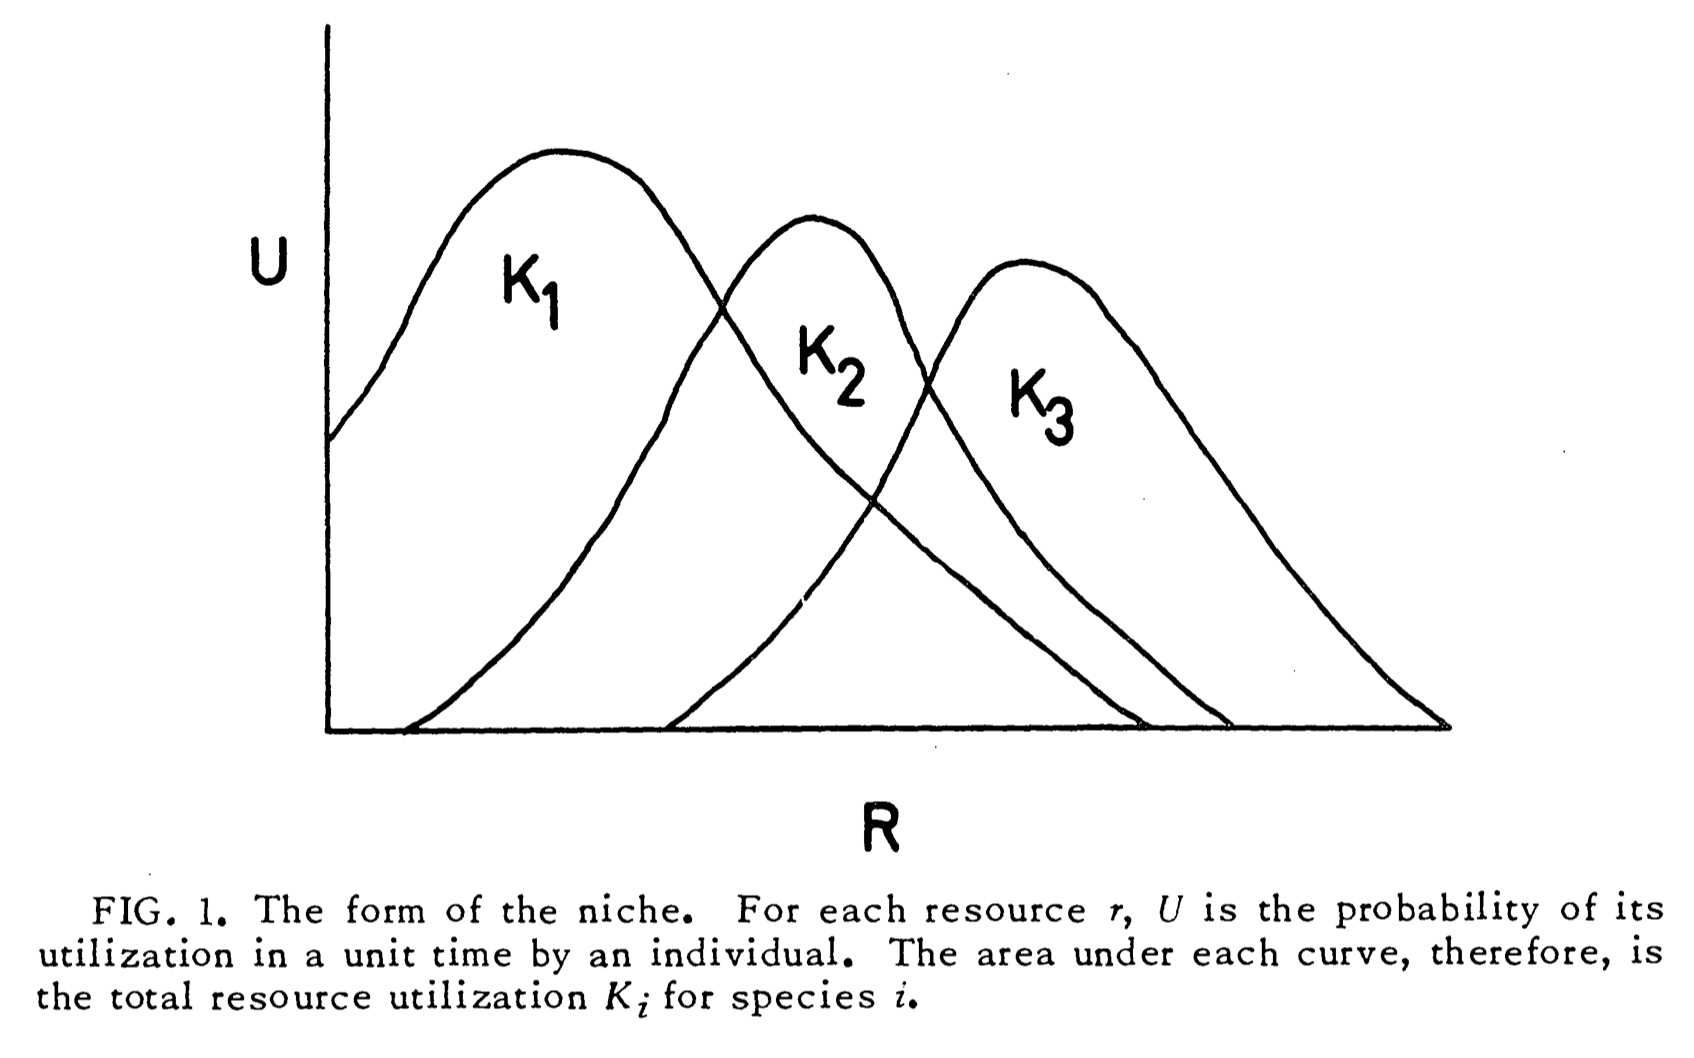
\includegraphics[width=.8\textwidth]{pics/limiting_similarity.png}
    
%     \small ``Limiting similarity'' --- MacArthur and Levins 1967
%   \end{center}
% \end{frame}

% % http://geology.gsapubs.org/content/30/1/15/F1.expansion.html
% \begin{frame}[t]{Competition and coexistance}
%   \begin{center}
%     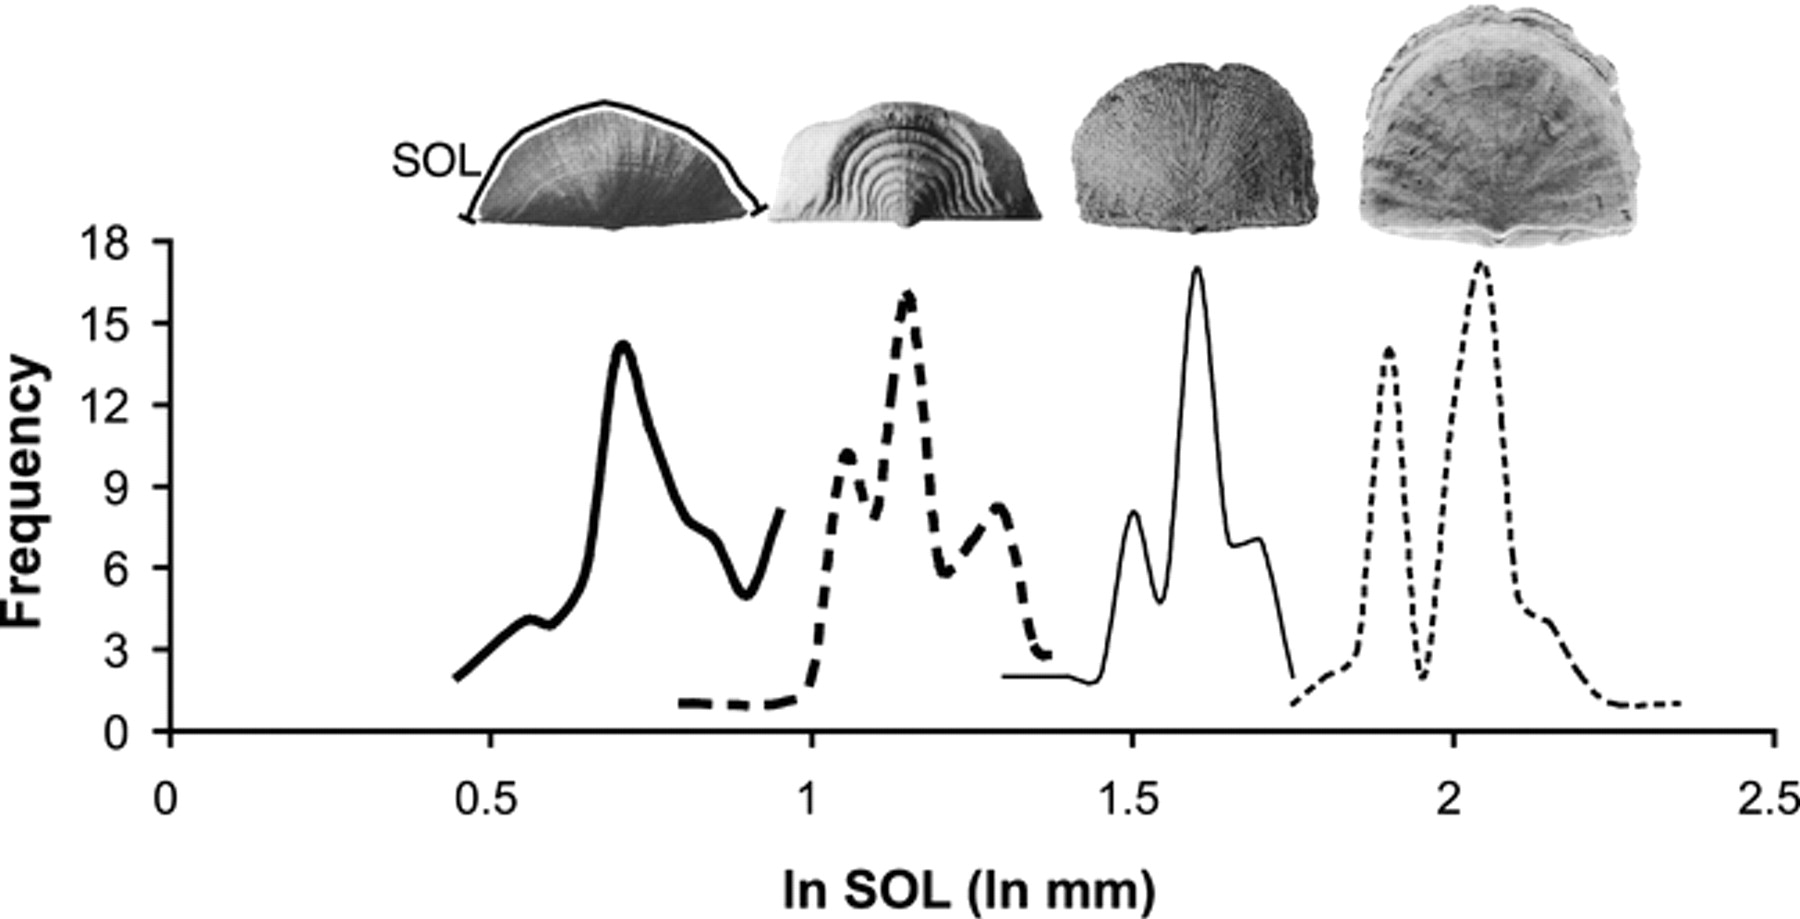
\includegraphics[width=.8\textwidth]{pics/hermoyian-2002.jpg}
    
%     Hermoyian et al. 2002
%   \end{center}
% \end{frame}

% \begin{frame}[t]{Character displacement}
%   \begin{center}
%     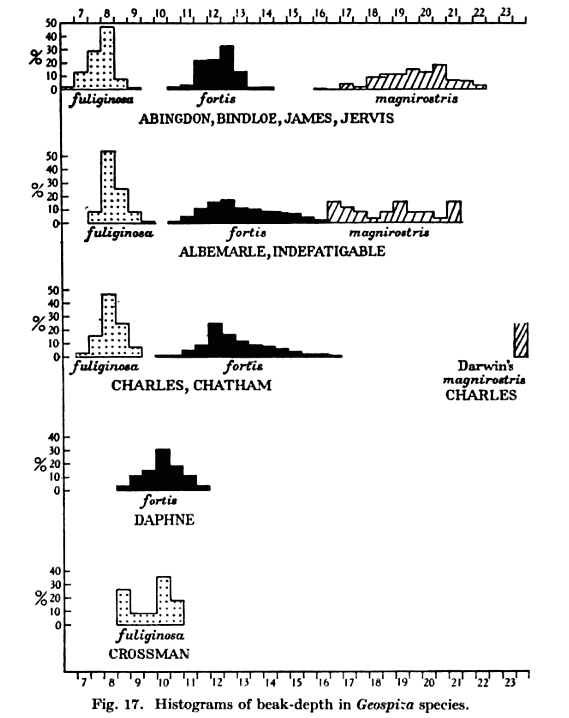
\includegraphics[height=.8\textheight]{pics/finches}

%     \small Lack 1947
%   \end{center}
% \end{frame}

% \begin{frame}[t]{Aims:~~~proximate aim}
%  Measure the shape of competition with respect to traits.
%  \begin{itemize}
%  \item ``Competition kernel''
%  \item In models mostly, but possibly in biological data
%  \item Qualitatively: symmetric, asymmetric?
%  \item Variation with abundance: linear, saturating, accelerating?
%  \item In models with known kernels
%  \end{itemize}
% \end{frame}

% \begin{frame}[t]{Aims:~~~ultimate aim \& implications}
%  \begin{itemize}
%  \item How reasonable are commonly used
%    functions?
%    \begin{itemize}
%    \item Key ingredient for models of coexistence, population
%      dynamics, evolution of traits, character displacement, etc.
%    \end{itemize}
%  \item What are experiments that measure competition really
%    measuring?
%  \item Coexistence question: do different competition kernels lead
%    to different patterns of coexistence?
%    \begin{itemize}
%    \item Leimar et al. approach answered some of this
%    \item Interaction with ``carrying capacity'' important
%    \item Competition appears not sufficient information to determine
%      patterns of coexistence.
%    \end{itemize}
%  \item Which types of factors generate symmetry/asymmetry in
%    competition?
%  \end{itemize}
% \end{frame}


% \begin{frame}[t]{Approach}
%   \begin{itemize}
%   \item Think about what competition \emph{means}
%   \item Start with models with ``explicit competition'' and recover
%     this
%     \begin{itemize}
%     \item Models where the competition function is baked directly into
%       the model - if we know what it is already, should be able to
%       recover it as a test case.
%     \end{itemize}
%   \item Next, relatively simple models with ``implicit competition''.
%     \begin{itemize}
%     \item Models where competition \emph{emerges}, e.g., via shared
%       resource use.
%     \end{itemize}
%   \item Complicated mechanistic models with implicit competition based
%     on things we know about species
%     \begin{itemize}
%     \item Starting with Daniel's vegetation model.
%     \end{itemize}
%   \end{itemize}
% \end{frame}

% \begin{frame}[t]{Simple models}
%   \begin{itemize}
%   \item Explicit competition:
%       \begin{itemize}
%       \item Dieckmann and Doebeli 1999: symmetric Gaussian competition\\
%         (speciation by disruptive selection)
%       \item Kisdi 1999: Asymmetric (logistic) competition\\
%         (evolutionary arms races)
%       \end{itemize}
%   \item Implicit competition:
%       \begin{itemize}
%       \item Tilman 1982 (\& various) \Rstar model\\
%         Shared use of resources
%       \end{itemize}
%   \item Mechanistic competition:
%     \begin{itemize}
%     \item Falster 2010/2014\\
%       Forest stand with competition for light
%     \end{itemize}
%   \end{itemize}
% \end{frame}

% \begin{frame}[t]{Dieckmann and Doebeli 1999 \subt{Gaussian}}
%   \begin{itemize}
%     \item Key features:
%       \begin{itemize}
%       \item Competition reduces a species carrying capacity via a
%         Gaussian function, and is \textbf{symmetric} (e.g., similar
%         species compete more strongly than dissimilar species).
%       \item Species effects are linear with respect to density
%       \item Carrying capacity is also Gaussian
%       \end{itemize}
%     \item Other similar models: Doebeli and Dieckmann (2010; Am Nat),
%       Case and Taper (2000; Am Nat) / Goldberg and Lande (2010; Am
%       Nat), Leimar et al. (2013; J Theor Biol)
%       \begin{itemize}
%       \item some of these have competition affecting growth rate,
%         rather than carrying capacity
%       \end{itemize}
%     \item Doebeli and Ispolatov (2013; Math Biol) argue these are
%       very general, even out to models where competition is really
%       asymmetric.
%   \end{itemize}
% \end{frame}

% \begin{frame}[t]{Gaussian competition \subt{Dieckmann and Doebeli 1999}}
%   \only<1>{\wikipic{dieckmann__dd_competition_true}}
%   \only<2>{\wikipic{dieckmann__dd_carrying_capacity}}
% \end{frame}

% \begin{frame}[t]{Gaussian competition \subt{Dieckmann and Doebeli 1999}}
%   Fitness:

%   \begin{center}
%     \begin{displaymath}
%       w(x^\prime, x, y) = 
%       r\left(1 - \frac{\sum_{i=1}^N
%           N_i \, {\color{red}\exp\left(-\frac{(x^\prime-x_i)^2}{2\sigma_C^2}\right)}}
%         {K_0 \exp \left(-\frac{{x^\prime}^2}{2\sigma_K^2}\right)}
%       \right)
%     \end{displaymath}
%   \end{center}
% \end{frame}

% \begin{frame}[t]{Gaussian competition \subt{Dieckmann and Doebeli 1999}}
%   Fitness:
%   \wikipic{dieckmann__dd_fitness_landscape}
% \end{frame}

% \begin{frame}[t]{Kisdi 1999 \subt{Asymmetric}}
%   \begin{itemize}
%     \item Key features:
%       \begin{itemize}
%       \item Competition reduces a species growth rate via a logistic
%         function, and is \textbf{asymmetric} (e.g., larger species are
%         competitively superior)
%       \item Species effects are linear with respect to density
%       \item Carrying capacity is linear (in opposite direction to
%         competitive hierarchy) or Gaussian.
%       \end{itemize}
%     \item Similar models include Geritz et al. (1999; Theor Pop Biol)
%       for seed size.
%     \item Less common than symmetric models
%   \end{itemize}
% \end{frame}

% \begin{frame}[t]{Asymmetric \subt{Kisdi 1999}}
%   \wikipic{kisdi__k_competition_felt}
% \end{frame}

% \begin{frame}[t]{Asymmetric \subt{Kisdi 1999}}
%   \begin{itemize}
%   \item Note that this is competition \textbf{felt}
%   \item Species with low trait values have their growth suppressed by
%     bigger species, but that is compensated by a higher intrinsic
%     growth rate (I think mathematically similar to the carrying
%     capacity?)
%   \item In contrast, competition exerted:
%   \end{itemize}
% \end{frame}

% \begin{frame}[t]{Asymmetric \subt{Kisdi 1999}}
%   \wikipic{kisdi__k_competition_true}
% \end{frame}

% \begin{frame}[t]{Asymmetric \subt{Kisdi 1999}}
%   Fitness:
%   \begin{displaymath}
%       w(x^\prime, x, y) = 
%       \rho(x) - 
%         \sum_{i=1}^N N_i \,
%         {\color{red}\alpha(x_i - x_j)}
%   \end{displaymath}
%   \begin{displaymath}
%       w(x^\prime, x, y) = 
%       \rho(x) - 
%         \sum_{i=1}^N N_i \,
%         {\color{red}c\left(
%             1 - \frac{1}{1 + \exp(-k(x_i - x_j))}
%             \right)}
%   \end{displaymath}
% \end{frame}

% \begin{frame}[t]{Asymmetric \subt{Kisdi 1999}}
%   Fitness:
%   \only<1>{\wikipic{kisdi__k_fitness_landscape}}
%   \only<2>{\wikipic{kisdi__k_fitness_landscape_detail}}
% \end{frame}

% \begin{frame}
%   \large
%   If all we can use is the fitness function, how do we infer the shape of
%   competition?

%   \pause
%   \vspace{1em}
%   Sensitivity of fitness to resident density

%   \begin{displaymath}
%     \left. \frac{d w_i}{d N_j} \right|_{N_i = 0, N_j = \hat N_j}
%   \end{displaymath}

%   \pause
%   \vspace{1em}
%   If increasing density of resident decreases invader fitness, the
%   invader is being competed against by the resident.
% \end{frame}

% \begin{frame}[t]{Fitness Jacobian}
%   \only<1>{\wikipic{dieckmann__dd_mutant_1}}
%   \only<2>{\wikipic{dieckmann__dd_mutant_2}}
%   \only<3>{\wikipic{dieckmann__dd_mutant_2_slope}}
%   \only<4>{\wikipic{dieckmann__dd_derivative}}
%   \only<5>{\wikipic{dieckmann__dd_derivative_scaled}}
%   \only<6>{\wikipic{kisdi__k_derivative}}
% \end{frame}

% \begin{frame}[t]{Tilman 1982\subt{R star}}
%   \begin{itemize}
%   \item Key features:
%     \begin{itemize}
%     \item No explicit competition kernel, no explicit carrying
%       capacity
%     \item Species consume shared resources at some rate and convert
%       them into offspring
%     \item Externally specified rate of resource regeneration
%     \item For k resources, up to k species can coexist
%     \item Species ``draw down'' resources to their \Rstar; species
%       with higher requirements die.
%     \end{itemize}
%   \item Terrifying literature of variants and tweaks
%   \item Probably the simplest possible shared resource model
%   \item Considering single resource case here (one winner)
%   \end{itemize}
% \end{frame}

% \begin{frame}[t]{R star \subt{Tilman 1982}}
%   Fitness, with respect to parameter affecting rate of conversion to
%   new offspring (bigger K, more required)
%   \wikipic{rstar_1__r1_fitness_landscape_K}
% \end{frame}

% \begin{frame}[t]{R star \subt{Tilman 1982}}
%   As a function of resident density
%   \wikipic{rstar_1__r1_mutant_1}
% \end{frame}

% \begin{frame}[t]{R star \subt{Tilman 1982}}
%   Invader fitness sensitivity to resident:
%   \only<1>{\wikipic{rstar_1__r1_mutant_1_slope}}
%   \only<2>{\wikipic{rstar_1__r1_derivative}}
% \end{frame}

% \begin{frame}[t]{R star \subt{Tilman 1982}}
%   \begin{itemize}
%   \item This is confusing:
%     \begin{itemize}
%     \item Species with low K values who will replace the resident are
%       most strongly competed against by the resident.
%     \item But these species also have the highest \textbf{potential}
%       fitness
%     \end{itemize}
%   \end{itemize}
% \end{frame}

% \begin{frame}[t]{R star \subt{Tilman 1982}}
%   Fitness in empty environment:
%   \wikipic{rstar_1__r1_fitness_empty}
% \end{frame}

% \begin{frame}[t]{R star \subt{Tilman 1982}}
%   Scale $w$ to get $w / w_{max}$ and take derivative of \emph{that}:
%   \wikipic{rstar_1__r1_derivative_scaled}
% \end{frame}

% \begin{frame}[t]{R star \subt{Tilman 1982}}
%   Competition stronger, and more trait dependent under low resources
%   \wikipic{rstar_1__r1_derivative_scaled_S}
% \end{frame}

% % Hmm - looks like the point where competition becomes non-unimodal in
% % density is at the resident density equilibrium.  That's interesting.
% \begin{frame}[t]{R star \subt{Tilman 1982}}
%   Nonlinear competition with density
%   \only<1>{\wikipic{rstar_1__r1_mutant_1_slope}}
%   \only<2>{\wikipic{rstar_1__r1_fitness_varying}}
%   \only<3>{\wikipic{rstar_1__r1_fitness_varying_scaled}}
%   \only<4>{\wikipic{rstar_1__r1_derivative_varying_scaled}}
%   \only<5>{\wikipic{rstar_1__r1_derivative_varying_scaled_twice}}
%   \only<6>{\wikipic{rstar_1__r1_derivative_scaled_twice_image}}
%   \only<7>{\wikipich{rstar_1__r1_derivative_scaled_twice_3d}}
% \end{frame}

% \begin{frame}[t]{Where next?}
%   \begin{itemize}
%   \item Is this a sensible measure?  Seems very sensitive to scaling,
%     and negative ``potential fitness'' causes real problems.
%   \item R star 2 resource model (really weird)
%   \item Falster 2010/2014 (really, really weird)
%   \item What do these mean for Lotka-Volterra models?
%   \item Age structured models
%   \item Multiple residents and the other linear assumption
%   \item Connection with empirical literature - \textbf{curvature} of
%     density is used there.
%   \end{itemize}
% \end{frame}

\end{document}

%%% Local Variables: 
%%% mode: latex
%%% TeX-PDF-mode: t
%%% TeX-engine: xetex
%%% End: 

%  LocalWords:  Tilman Dieckmann Lande Leimar Theor Ispolatov Geritz
%  LocalWords:  dieckmann kisdi Jacobian rstar Lotka Volterra
